\section{Results}

\begin{figure}[h]
    \centering
    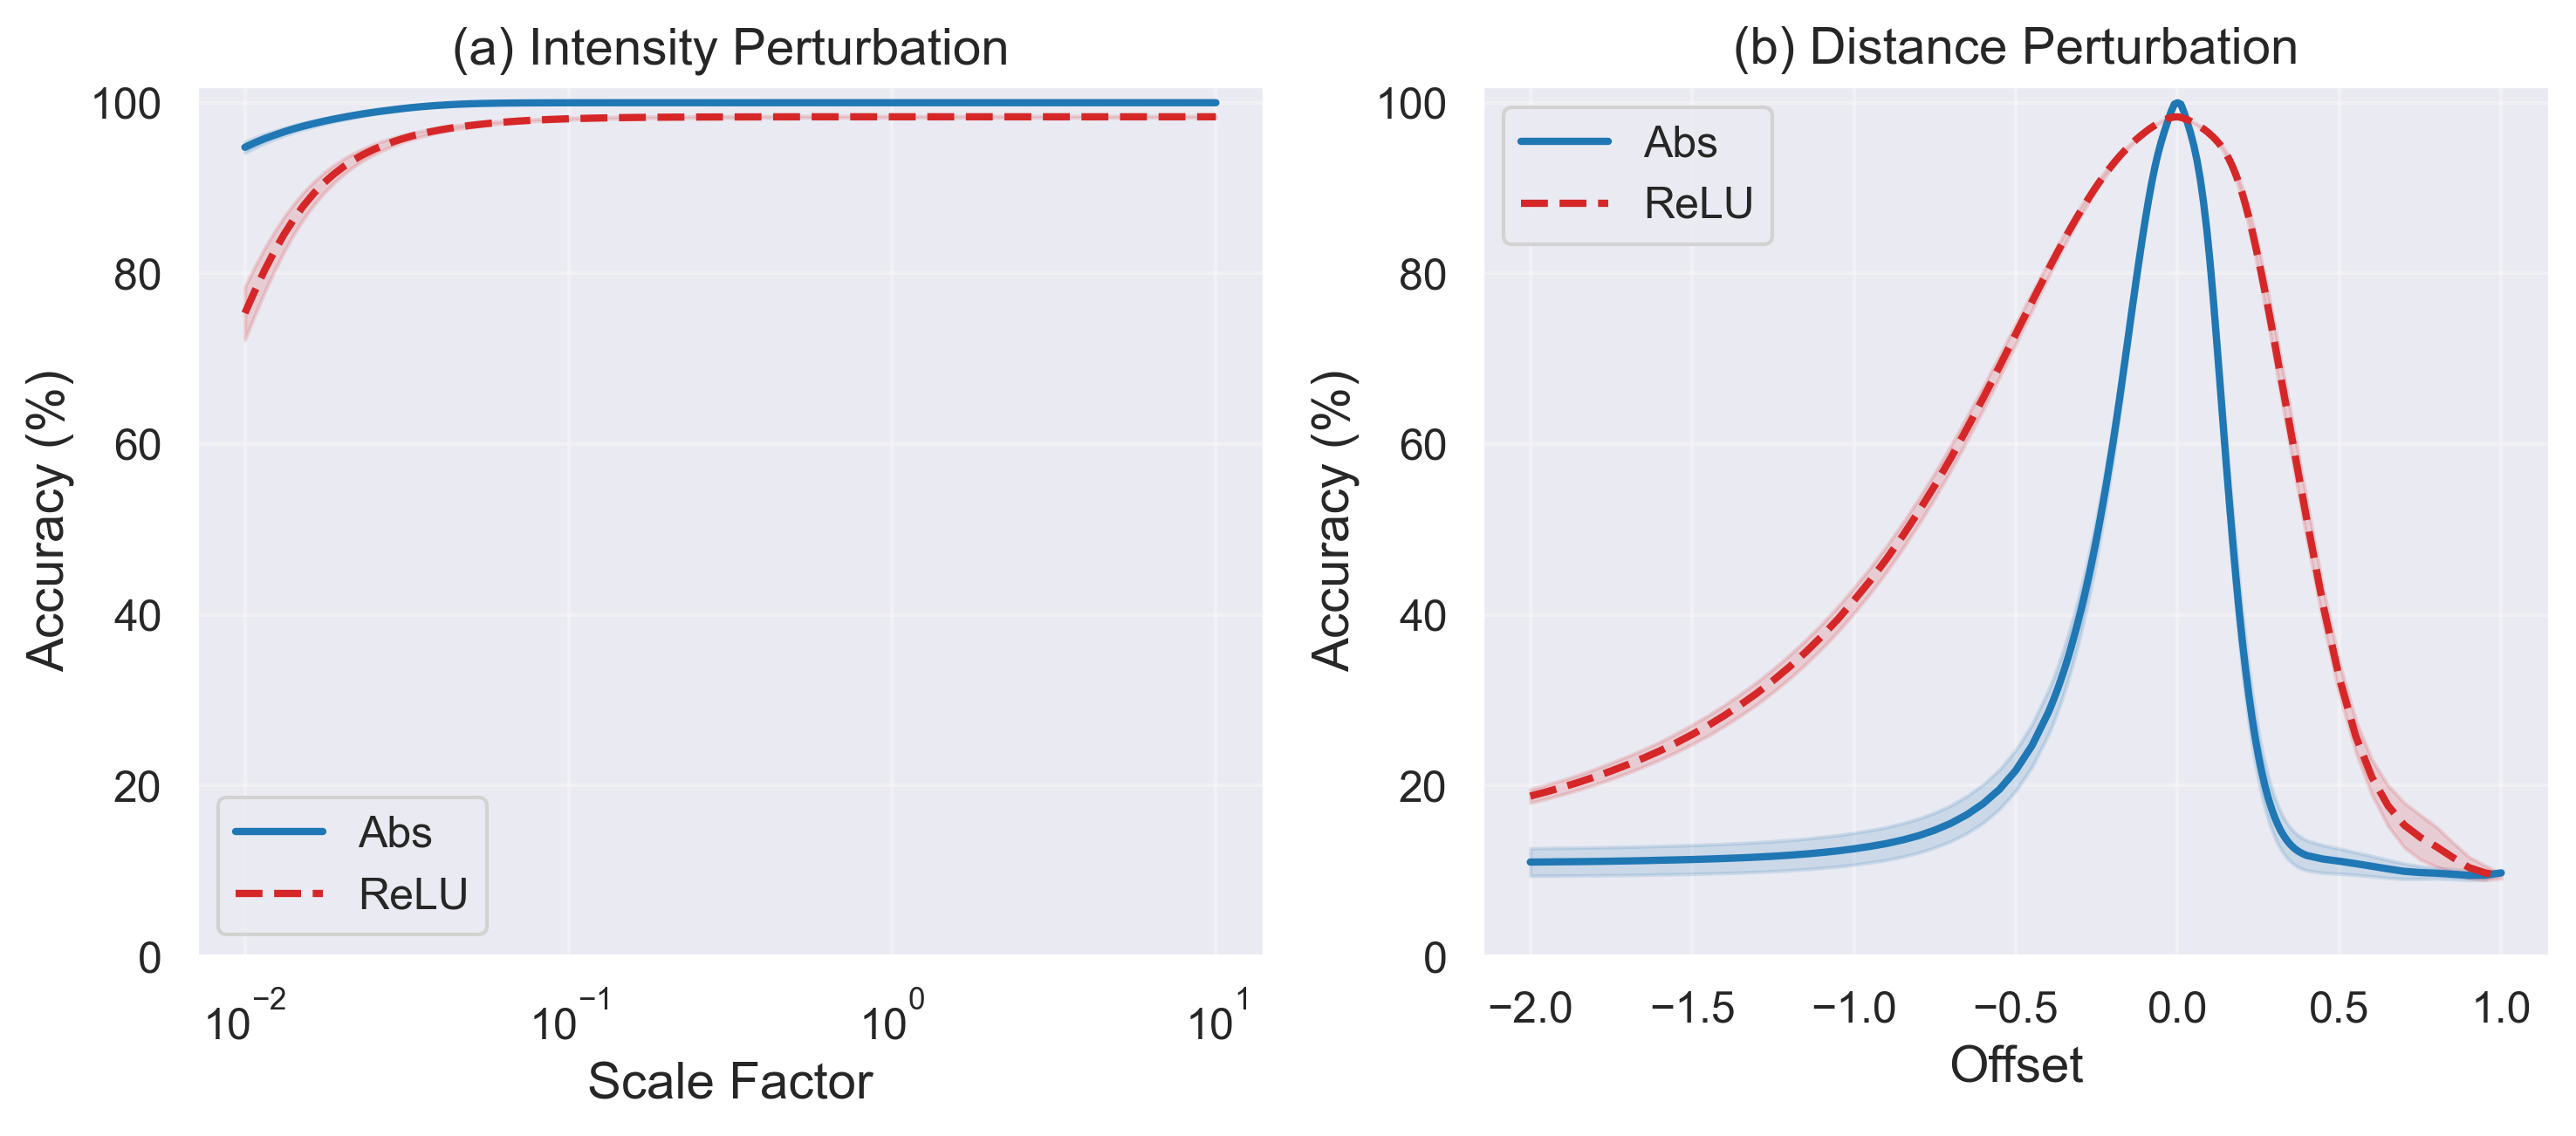
\includegraphics[width=\textwidth]{images/perturbation_analysis}
    \caption{Effects of intensity scaling and distance offset perturbations on model accuracy. Shaded regions represent 95\% confidence intervals across 20 runs.}
    \label{fig:perturbation_analysis}
    \end{figure}
\subsection{Statistical Analysis}

    

Results of the experiment provide strong empirical support for our theory that the tested models primarily utilize distance metrics rather than intensity metrics.

\begin{table}[h]
    \centering
    \begin{tabular}{lrrr}
    \hline
    Model & Training Acc (\%) & Test Acc (\%) & Loss \\
    \hline
    Abs & 99.99 $\pm$ 0.00 & 95.29 $\pm$ 0.20 & 0.0047 $\pm$ 0.0005 \\
    ReLU & 98.33 $\pm$ 0.15 & 95.61 $\pm$ 0.14 & 0.0610 $\pm$ 0.0044 \\
    \hline
    \end{tabular}
    \caption{Baseline model performance averaged across 20 training runs (mean $\pm$ standard deviation).}
    \label{tab:baseline}
\end{table}

Both models achieved strong classification performance on MNIST before perturbation testing, as shown in Table~\ref{tab:baseline}.

Both models demonstrate strong invariance to intensity perturbations while showing significant sensitivity to distance perturbations, supporting our theory. Figure~\ref{fig:perturbation_analysis} shows these effects across perturbation types.

Both models maintain their baseline accuracy (98\% for ReLU and 99\% for Abs) across both scaling (10\% to 200\% of output ranges) and threshold clipping (50\% and above). The minimal drop in performance is small and statisticaly significant (p < 0.01). 

Both models lose accuracy quickly with small offset perturbations. ReLU maintains its baseline of 98\% over a -3\% to +2\% offset range. Abs is even more sensitive and falls below 99\% outside of -1\% to +1\%.

Most of these values are highly statistically significant as shown in Table~\ref{tab:scale_data},  Table~\ref{tab:clip_data}, and  Table~\ref{tab:distance_data}.

\begin{table}[h]
    \centering
    \begin{tabular}{lrrrrrr}
    \hline
    Change & Abs Acc (\%) & Abs T & Abs P & ReLU Acc (\%) & ReLU T & ReLU P \\
    \hline
    +10\% & 99.98 & 5.460 & 2.879e-05 & 98.10 & 10.374 & 2.906e-09 \\
    +20\% & 99.98 & 0.845 & 4.085e-01 & 98.29 & 6.520 & 3.029e-06 \\
    +40\% & 99.99 & -0.566 & 5.779e-01 & 98.33 & -4.334 & 3.578e-04 \\
    +80\% & 99.99 & -1.674 & 1.106e-01 & 98.33 & -3.514 & 2.320e-03 \\
    +900\% & 99.99 & -2.015 & 5.829e-02 & 98.33 & -3.202 & 4.693e-03 \\
    \hline
    \end{tabular}
    \caption{Results for intensity scale perturbations compared to baseline performance.}
    \label{fig:scale_data}
\end{table}
    
\begin{table}[h]
    \centering
    \begin{tabular}{lrrrrrr}
    \hline
    Change & Abs Acc (\%) & Abs T & Abs P & ReLU Acc (\%) & ReLU T & ReLU P \\
    \hline
    +10\% & 71.05 & 21.910 & 6.030e-15 & 87.56 & 22.964 & 2.547e-15 \\
    +20\% & 88.55 & 20.972 & 1.342e-14 & 93.84 & 20.603 & 1.855e-14 \\
    +40\% & 98.70 & -25.278 & 4.344e-16 & 97.74 & -23.404 & 1.796e-15 \\
    +80\% & 99.98 & -26.454 & 1.873e-16 & 98.33 & -27.941 & 6.789e-17 \\
    \hline
    \end{tabular}
    \caption{Results for intensity clip perturbations compared to baseline performance.}
    \label{fig:clip_data}
\end{table}

\begin{table}[h]
    \centering
    \begin{tabular}{lrrrrrr}
    \hline
    Change & Abs Acc (\%) & Abs T & Abs P & ReLU Acc (\%) & ReLU T & ReLU P \\
    \hline
    -80\% & 14.14 & 47.472 & 3.309e-21 & 52.11 & 63.948 & 1.191e-23 \\
    -20\% & 60.05 & -28.028 & 6.410e-17 & 80.38 & 40.709 & 5.973e-20 \\
    -10\% & 86.25 & -31.506 & 7.260e-18 & 92.78 & -33.276 & 2.616e-18 \\
    -4\% & 96.73 & -40.478 & 6.644e-20 & 96.55 & -36.744 & 4.088e-19 \\
    -1\% & 99.82 & -42.731 & 2.400e-20 & 97.98 & -38.915 & 1.393e-19 \\
    +1\% & 99.81 & -42.727 & 2.405e-20 & 98.31 & -39.848 & 8.924e-20 \\
    +4\% & 96.45 & -39.975 & 8.406e-20 & 98.26 & -39.645 & 9.821e-20 \\
    +10\% & 81.40 & -19.541 & 4.856e-14 & 97.81 & -37.453 & 2.857e-19 \\
    +20\% & 36.90 & 7.887 & 2.068e-07 & 96.31 & -28.323 & 5.277e-17\\
    +80\% & 9.74 & 45.298 & 8.004e-21 & 12.83 & 70.202 & 2.038e-24 \\
    \hline
    \end{tabular}
    \caption{Results for distance perturbations (offset) compared to baseline performance.}
    \label{fig:distance_data}
\end{table}

